\documentclass{article}
\usepackage[T1]{fontenc}
\usepackage{lmodern}
\usepackage{graphicx}
\usepackage{amsmath,amssymb}
\usepackage[a4paper,margin=2cm]{geometry}
\usepackage[absolute,overlay]{textpos}
\setlength{\TPHorizModule}{1mm}
\setlength{\TPVertModule}{1mm}
\usepackage[indonesian]{babel}
\usepackage{hyperref}
\setlength{\emergencystretch}{2em}
% unit: Halaman 56

\begin{document}

% === Halaman 56 (llm) ===

\begin{itemize}
    \item Misalnya jika terdapat 64 $byte$ dan 15 bit pesan yang akan disembunyikan. $Pixel-pixel$ dipilih secara acak, seperti pada gambar berikut.
\end{itemize}

\vspace{10mm}

% deskripsi: Grid 8x8 yang merepresentasikan pixel-pixel, dengan beberapa sel berisi angka yang menunjukkan urutan pemilihan pixel secara acak untuk menyembunyikan bit pesan.
% bbox normalisasi: [0.3130, 0.4080, 0.6030, 0.8310]
\begin{textblock*}{60.90mm}(65.73mm,121.18mm)
\noindent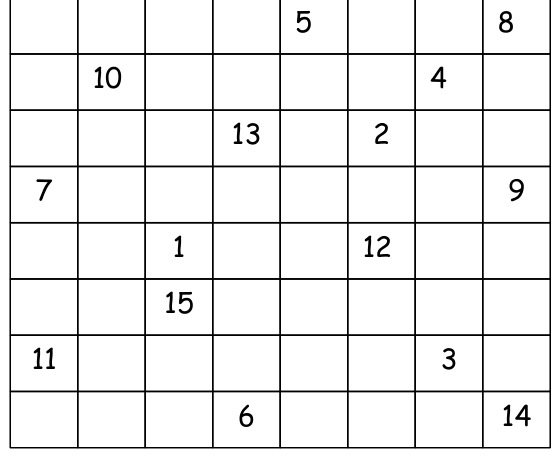
\includegraphics[width=60.90mm,height=125.63mm]{../../images/llm/page_056_img_01.png}%
\end{textblock*}

\end{document}
